\section{Wi-fi Protected Access and Temporal Key Integrity Protected}

\ac{WPA} is a security protocol in \ac{WLAN} developed by Wi-fi Alliance to secure \ac{WLAN}. Officially adopted by \ac{IEEE}802.11 in 2003 \cite{1318903}, this protocol is based on \ac{WEP} mechanism, but to offer an improvement over \ac{WEP} vulnerability. Both \ac{WPA} and \ac{WEP} uses the same encryption and decryption key, yet \ac{WPA} use \ac{TKIP} which is dynamically changed while in use \cite{wpa(wi-fiprotectedaccess)definition}. Moreover, \ac{WPA} deploys \ac{EAP} to authenticate user instead of using only \ac{MAC} address. The use of \ac{EAP} circumvents the attacker from getting authorized to gain access to the wireless network.

\subsection{TKIP mechanism}
\ac{TKIP} is the core of \ac{WPA} which works on the same existed hardware with \ac{WPA}. The improvement, provided by \ac{TKIP}, chiefly focuses on software improvement. As a result, \ac{TKIP} could not overcome the hardware constraint to provide an entirely safe \ac{WLAN} environment. As a short-term solution, \ac{TKIP}, however, is an economical and feasible improvement on \ac{WEP} \cite{al2006ieee}.

\ac{TKIP} still bases on \ac{RC4}, but uses a longer \ac{IV} and encryption and decryption key compared to \ac{WEP}. It deploys $48 bits$ \ac{IV}, $64 bits$ authentication and $128 bits$ encryption key(or \ac{TK}) \cite{potter2003wireless}. There are $2^{48}$ possible \ac{IV} which is a large number compared to $2^24$ IV's in traditional \ac{WEP}. The long \ac{IV} and encryption key make \ac{TKIP} be more secure against exhaustive search. Furthermore, \ac{TKIP} use different keys per packer which effectively avoids key reuse.

In \cite{doomun2012modified}, \citeauthor{doomun2012modified} described two phases to construct the key used in message encryption.

The first phase mixes $128 bits$ \ac{TK} with the first $32 bits$ of \ac{IV} and $48 bits$ of \ac{MAC} address of a transmitter device. The output of this step is an immediate key called \ac{P1K}. In this phase, a $48 bits$ \ac{MAC} address of transmitter device is used to do \ac{Xor} operation with $128 bits$ \ac{TK} iteratively. The result is divided into a number of bytes and each one is used to index an S-box, which is an invertible non-linear substitution table, to give out $80 bits$ intermediate key \ac{P1K}. \ac{P1K} is computed every $2^{16}$ packets and would be cached to alleviate overheats in network performance. Mixing \ac{MAC} address into \ac{P1K} guarantees that different devices or \ac{AP}s would results in different \ac{P1K}. As a result, this phase thwarts attackers from using key stream reuse due to cross-station \ac{IV} collision. 

The second phase takes input as $80 bits$ \ac{P1K} with $128 bits$ \ac{TK} and the $16$ least significant $bits$ of \ac{IV}. The output of this phase is unique $128 bits$ \ac{RC4} key. In this step, \ac{TKIP} utilise S-box substitution, rotate operation and addition to calculate \ac{RC4} key for every packet. This close the association between \ac{IV} and the key. Thus, it is able to circumvent the attacker from exploiting  keys to recover \ac{TK}.

After we get $128 bits$ \ac{RC4}, this would be divided into \ac{WEP} \ac{IV}-$24 bits$ and \ac{WEP} \ac{IV}-$104 bits$ then transmits following \ac{WEP} algorith. The detail of \ac{TKIP} process is described in \autoref{fig:tkip} %ref hinh vao%

\begin{figure}
	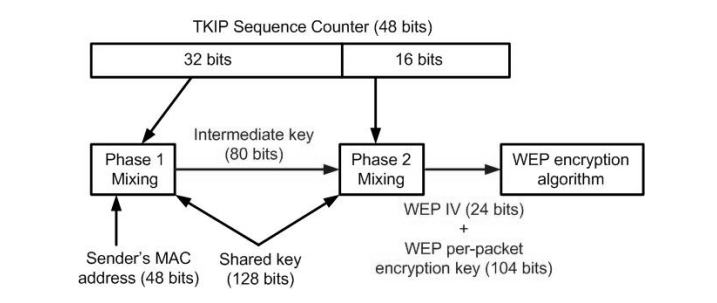
\includegraphics[scale=0.45]{images/tkip.png}
	\caption{\ac{TKIP} construction}
	\label{fig:tkip}
\end{figure}

Another strength of \ac{TKIP} is a cryptographic protocol called \ac{MIC} \cite{1318903}. \ac{MIC} employs a cryptographic one way hash function. This functions receive the inputs as $64 bits$ authentication key and the message. After that, several logic operations such as \ac{Xor}, bit swapping and bit addition is employed to produce a special tag of the message as an output. On receiver device, a verification procedure is used to generate a tag from message and check if the generated tag is exactly similar to the transmitted tag. If two tags are matched, that means the original message is not modified. Adversely, the message has been tampered. The operation of \ac{MIC} is described in \autoref{fig:mic}  %cite hinh vao%.



\subsection{TKIP shortcomings}
Although, there are several work to ameliorate \ac{TKIP} \cite{doomun2012modified}. However, as above discussion, \ac{TKIP} is an updated software of \ac{WEP}. It can not overcome the constraint of hardware. The use of \ac{RC4} is still a weakness of \ac{TKIP} as \ac{RC4} is still considered as an weak encryption method. Furthermore, \ac{TKIP} users would endure the low performance of network due to its expensive encryption computation for every packet. 

\subsection{Summary}
In general, \ac{TKIP} is not a long-term solution for \ac{WLAN}. The further development for a safe alternative for \ac{WEP} or \ac{TKIP} might require both hardware change and protocols as well.

\begin{figure}
	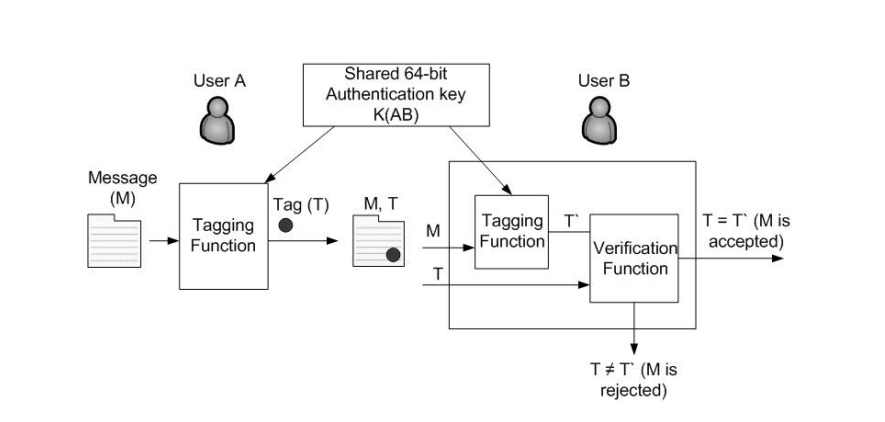
\includegraphics[scale=0.4]{images/mic.png}
	\caption{\ac{MIC} operation}
	\label{fig:mic}
\end{figure}